% Custom title page for Quarto PDF output.
% Included via YAML: include-before-body: file: titlepage.tex

\newgeometry{top=10mm, bottom=10mm, inner=20mm, outer=20mm}

\begin{titlepage}
\begin{flushleft}

\includegraphics[width=0.25\paperwidth]{graphics/schoolLogo}
\end{flushleft}

\vspace*{0.1\textheight}

\begin{center}
\textsf{Labbrapport}
\end{center}

\vspace{0.03\textheight}

\begin{spacing}{1.4}
\begin{center}
\textsf{\textbf{\huge Labbpaket 1}}
\end{center}
\end{spacing}

\vspace{0.03\textheight}

\begin{singlespace}
\begin{center}
\textsf{Förnamn Efternamn, Förnamn Efternamn, Förnamn Efternamn}
\vspace{0.03\textheight}
\end{center}
\end{singlespace}

\begin{center}
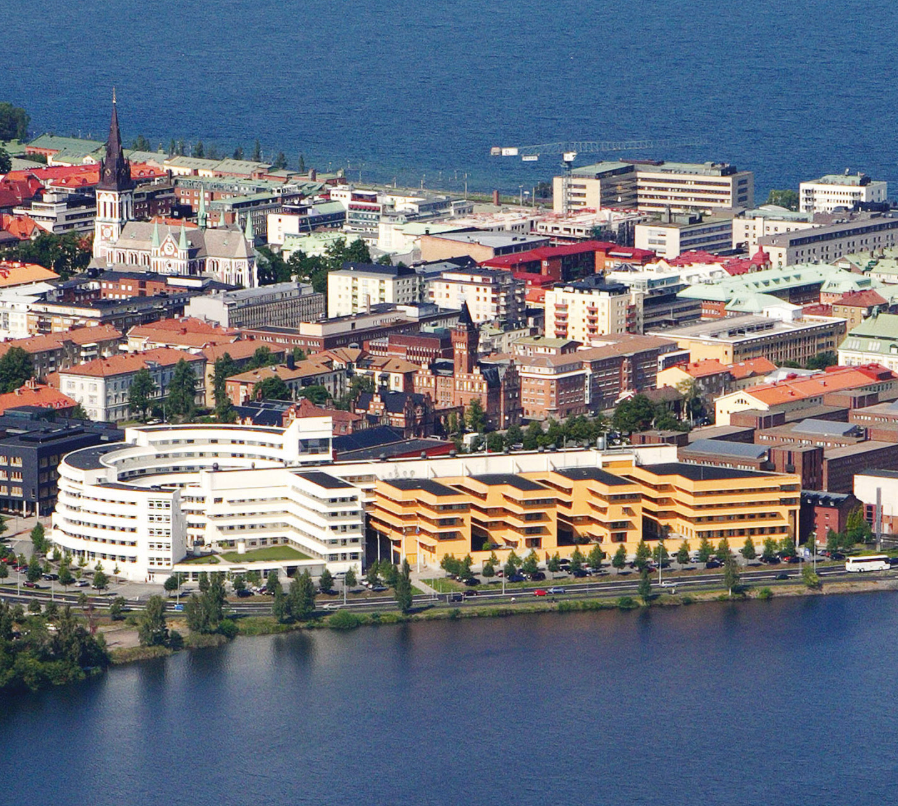
\includegraphics[width=0.35\paperwidth]{graphics/jupic}
\end{center}

\vspace{0.1\textheight}

\begin{center}
\textsf{v. 1.0}
\end{center}

\vfill

\begin{flushleft}
\textsf{Jönköping University}\\
\textsf{School of Engineering}\\
\textsf{Mechanical Engineering \textbullet{} 2026}
\end{flushleft}

\end{titlepage}

\restoregeometry
